% Remember to input this to the presentative tex file before compiling.
\chapter{Neural Networks Based Classifiers}

Classification problems for a complex and large dataset with unpredictable results using linear methods can be calculated using neural networks, which can be trained to adjust with the result requirements. Also, once we train the network, it can be used on any similar dataset efficiently and with higher accuracy. Neural networks are just a set of functions that change themselves to learn and fit into a model. 

\section{How Neural Networks Works}
Neural networks are computational models inspired by the structure and function of the human brain. It consists of interconnected nodes in this case neurons, organized into layers. Each neuron receives input signals, processes them using an activation function, and produces an output signal. Layers are typically organized into an input layer, one or more hidden layers, and an output layer. The input layer receives raw data, while the output layer produces the model's predictions or classifications. There are hidden layers between the input and output layers, where the network learns to predict the result from the input data. Each connection between neurons is associated with weights, and each neuron also has a bias term. During training, the network adjusts these weights and biases using an optimization algorithm to minimize the loss function, which measures the difference between the predicted output and the true labels.\\
A neural network is trained by giving it labelled training data and modifying its weights and biases to reduce the difference between the labels it predicts and the actual labels. This is done through an iterative process of forward propagation, loss calculation, and backpropagation. In forward propagation, input data is passed through the network, layer by layer. At each layer, the input is transformed by the weights and biases of the neurons and then passed through the activation function to produce an output, and this Output becomes the Input of the next layer. This process continues until the output layer is reached, producing the model's prediction.
After getting the Output at the end of the last layer, the loss function is calculated by comparing the predicted output to the true labels or target values. Common loss functions are mean squared error for regression tasks and cross-entropy loss for classification tasks. The network then adjusts its weights and biases through backpropagation, by computing the gradient of the loss function with respect to each weight and bias in the network and updating them accordingly. This process continues for a predefined number of iterations (epochs) or until the model's performance on a separate validation dataset reaches a satisfactory level of result.

\section{Architecture of Neural Network}
A neural network consists of many neurons called nodes. Their amount could be from a couple of dozen to even millions, and they are arranged in layers. All the nodes can be classified into input, hidden, and output nodes, which connect the layers on either side. 

% picture workflow of neural network

The Input layer consists of input nodes responsible for receiving numerical data from outside of the dataset that the neural network attempts to learn about. The connection between one node from the input layer and one from the hidden layer is represented by a number called weight, which is denoted as $W_{i}$. The weight can be positive or negative, corresponding to how brain cells excite or suppress others. If a node has a higher corresponding weight, then it has more influence on the output. Initially, the weights are assigned randomly and are adjusted later in the training process.

In neural networks, information can flow through a neural network in two ways. The simplest type of Neural network is Feedforward Neural Network. In Feedforward Neural Network, the data value goes only in one direction, from the input nodes to hidden nodes, and then finally to the output nodes.
%Exapmle Picture of Feedforward Neural Networks

The Input layer Collects the numerical variables from the Dataset and carries them to the next stage, no computation happens here. Then, the data values are at the first hidden layer, which has an activation function. The activation functions perform computations and transfer the new values to the next hidden layer or output layer. A feedforward network will only have a single Input layer, and it can also have zero or multiple hidden layers.
The output layer contains all output nodes, which our results computed from prior hidden layers can be considered. One type of neural network, known as a recurrent neural network, has a loop or cycle connecting all the nodes inside it. The recurrent attribute allows it to exhibit temporal dynamic behaviours.


\subsection{Forward Neural Networks}
Neural networks refer to the complex links among neurons; communication links can join many neurons to carry out complex computations. The structure of a neural network can be described as a graph whose nodes are the neurons, and each edge in the graph links the output of one neuron to the input of another neuron. For the feed-forward network structure, the graph does not contain any loop.
A feed-forward neural network can be described by a directed acyclic graph, G = (V, E), and a weight function over the edges, $w: E\xrightarrow{}R$. Nodes of the graph can be considered as neurons. Each single neuron is moulded as a simple scalar function, $\sigma: R\xrightarrow[]{}R$.
$\sigma$ can be a 

sign function, $$\sigma(a) = sign(a)$$

threshold function, $$\sigma(a) = 1_{[a>0]}$$

the sigmoid function, $$\sigma(a) = \frac{1}{1+\exp{-a}}$$

The sigmoid function is a smooth approximation to the threshold function. $\sigma$ is called the "activation function" of the neuron.
Each edge in the graph links some neuron's output to another neuron's input. The input of a neuron is calculated by taking a weighted sum of the outputs of all the neurons connected to it, weighting can be tweaked by $w$.
Assume that the network is organized in \textit{layers}, that is, the set of nodes can be decomposed into a union of nonempty disjoint subsets, $V=\bigcup_{t=0}^{T}V_{t}$ (disjoint union), such that every edge in E connects some node in $V_{t-1}$ to some node in $V_{t}$, for some $t\in [T]$.

The bottom layer, $V_{0}$ is called the input layer. It contains n+1 neurons, where n is the dimension of the input space. For every $i\in[n]$, the output of neuron $i$ in $V_{0}$ is simply $x_{i}$.
The last neuron in $V_{0}$ is the "constant" neuron, which always outputs 1.

let's denote $v_{t,i}$ the $i$th neuron of $t$th layer
and $o_{t,i}(X)$ the output of $v_{t,i}$ when the network is fed with the input vector $x$.
Therefore, for $i\in[n]$ we have $o_{0,i}(x) = x_{i}$ and for $i = n+1$ we have$o_{0,i}(x)=1$.
Let's calculate in a layer-by-layer manner. Suppose we have already calculated the outputs of neurons at layer $t$.

Then, we can find the outputs of the neurons at layer $t+1$ by fixing some $v_{t+1,j}\in V_{t+1}$.
Let $a_{t+1,j}(x)$ denote the input to $v_{t+1,j}$ when the network is fed with the input vector $x$.

Then, $$a_{t+1,j}(x) = \sum_{r:(v_{t,r},v_{t+1,j})\in E}w((v_{t,r},v_{t+1,j}))o_{t,r}(x),$$ and $$o_{t+1,j}(x) = \sigma( a_{t+1,j}(x)) .$$

The input to $v_{t+1,j}$ is a weighted sum of the outputs of the neurons in $V_{t}$ that are connected to $v_{t+1,j}$, where weighting is according to $w$, and the output of $v_{t+1,j}$ is simply the application of the activation function $\sigma$ on its input.

Layers $V_{1},\cdots,V_{T-1}$ are often called \textit{hidden layers}. The top layer $V_{T}$ is called the Output Layer.
In Simple prediction problems, the output layer contains a single neuron whose output is the output of the network.

Let's Refer to $T$ as the number of layers in the network(excluding $V_{0}$) or the "depth" of the network. The size of the network $\mod{V}$. the "width" of the network is $max_{t}\mod{V_{t}}$. See Figure Below. A layered feedforward neural network of depth 2, size 10, and width 5 is given for better understanding.

Note that a neuron in the hidden layer has no incoming edges. this neuron will output the constant $\sigma(0).$

\subsection{Activation Function}
An activation function takes the dot-product mentioned before as an input and performs a certain computation on it.
A notable property of activation functions is that they should
be differentiable because this property is needed to train the neural network using backpropagation optimization.

\subsubsection{Sigmoid or Logistic}It takes a real-valued input and returns a output in range[0,1]
$$\delta(x)=\frac{1}{1+e^{-1}}$$ 
\textbf{sigmoid activation function picture}\\
In Fig, this is an S-shaped curve, and the values going through the Sigmoid function will be squeezed in the range of [0, 1]. Since the probability of anything exists only between the range of 0 and 1, Sigmoid is a compatible transfer function for probability. Although the Sigmoid function is easy to understand and ready to use, it is not used frequently because it has a vanishing gradient problem. This problem is that, in some cases, the gradient gets so close to zero that it does not effectively apply change to the weight. In the worst case, this may completely stop the neural network from further
training. Second, the output of this function is not zero-centered, which makes the gradient updates go far in different directions. Besides, the fact that output is in the narrow range [0, 1] makes optimization harder. In order to compensate for the shortcomings, the $tanh()$ function is an alternative option because it is a stretched version of the Sigmoid function, in which its output is zero-centred.
\subsubsection{$tanh$ or hyperbolic tangent:}
it takes real-valued input and produces the results in the range[-1,1]:
$$tanh(x) = \frac{\sinh{x}}{\cosh{x}}=\frac{e^{x}-e^{-x}}{e^{x}+e^{-x}}$$
The advantage is that the negative input values will be mapped strongly negative and zeros will be mapped near zero through this function. Therefore, this function is used when classification is needed to be performed between two classes. In practice, this function is preferred over the sigmoid function, but the gradient vanishing problem still exists. so the ReLU function is used
\subsubsection{ReLU} Rectified Linear Unit function takes a real-valued input and replaces the negative values with zero
$$R(x) = max(0,x)$$
The ReLU() activation function is trending now in the field of neural networks. It is used in almost all convolutional neural networks or deep learning because it is a relatively simple and efficient function that avoids and rectifies the gradient vanishing problem. The problem with this activation function is that all the negative values become zeros after this activation, which in turn affects the results by not taking negative values into account. A different activation function can be used when we know what characteristics of results we expect to see. Among these three activation functions, we usually start our training process using ReLU() because it works as a general approximator for most data sets.

\subsection{ Multi-Layer Perceptron} there are two types of feed-forward neural networks:
\begin{itemize}
    \item Single layer Perceptron: the simplest feed-forward neural network with no hidden layers.
    \item Multi-layer Perceptron: it has more than one layer, which is useful for practical application
\end{itemize}

Multi-layer perceptron can learn not only linear functions but also non-linear functions. The feed-forward neural network in Figure is an example of the multi-layer Perceptron. For a data set containing features and results, the multi-layer Perceptron will learn the relationship between features and results from the given data set and predict the result for
a new data point. Generally, in the input layer, we send n numerical inputs through n nodes:$$ x = x_{1},x_{2},\cdots,x_{n} |x\in R^{n}$$
then randomly assign weights for them in the first place: $$w = w_{1},w_{2},\cdots,w_{n}$$ the values for weights will be adjusted later in the training process for more accurate approximations.\\
In the hidden layer, all the inputs by taking the dot product of x and w, and is known as the pre-state P
$$P = w_{1}\cdot x_{1}+w_{2}\cdot x_{2}+\cdots+w_{n}\cdot x_{n}+b$$
$$ P = \sum^{n}_{i=1}(x_{i}w_{i}) + b$$

\begin{figure}
    \centering
    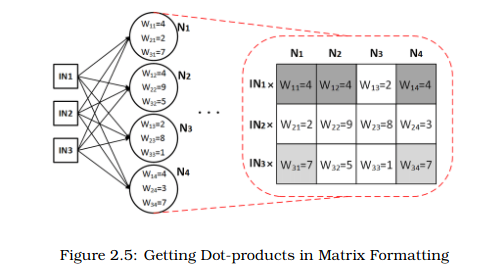
\includegraphics[width=0.6\linewidth]{Thesis Prashant//Images//media/Screenshot from 2024-04-23 00-29-37.png}
    \caption{Dot-products in Matrix Formatting}
    \label{fig:enter-label}
\end{figure}


Let's use vectors to represent them so that it can be treated as a matrix format. In Fig, the input layer has 3 nodes, and the following hidden layer has 4 nodes. Let's create a matrix of 3 rows and 4 columns and insert the values of each weight in the matrix as done above. This matrix would be called $W_{1}$. A 1 × 4 pre-state matrix can be obtained by matrix multiplication. In the hidden layer, four pre-states $N_{i}$, each store the dot-product of corresponding inputs and weights. These four pre-state values are ready to go through a certain activation function σ(). This is called the state S inside this hidden neuron.$$ S = \sigma(W_{i}IN_{i} +b)$$
There could be more hidden layers following the first hidden layer, and the state(s) S, which stores the transformed values, will be the input value(s) for the next layer. The matrix contains all the state values that will encounter the next weight matrix and produce new dot-products, and at that time, all the state values become the pre-state values of the next stage. The initial input values will go through every hidden layer in the neural net, repeat the same procedure mentioned above, and finally arrive at the output layer. The output values we receive are the ultimate state values in the very last hidden layer. This procedure explains how we set up our neural net.

%Now the question is, how do we determine the weights? How do we adjust the weights so that neural networks make more accurate predictions?

\subsection{Model Building}
A neural network learns from patterns of data and tries to make predictions as accurately as possible. Assume that we already have a set of $p$ data pairs containing the variables and the results, $(x^{(1)},t^{(1)}),(x^{(2)},t^{(2)}),\cdots, (x^{(p)},t^{(p)}),$ where $x^{(i)}$ is input value and $t^{(i)}$ is the target value for i=1, 2, 3, ..., p. We would like to build a neural net $F$ so that ideally, $$F(x^{(i)}) = t^{(i)}$$
typically for $\epsilon_{i}$. Let $y^{(i)}$ denote the output of the  neural network so that 
$$y^{(i)} =F(x^{(i)})  \text{ and } t^{(i)} = y^{(i)} + \Vec{\epsilon_{i}}$$
here $y^{(i)}$ depends on parameters, which are weights and biases, then it turns out as an optimization problem. so we need to set a neural network F that minimizes the error function, which is denoted by E
$$ E = \frac{1}{N} \sum_{i=1}^{p}||t^{(i)}-y^{(i)}||^{2}$$
where N is the number of training patterns. If it is a two-way classification problem, then N = 2. From this equation, E is a function of the parameters in F, and we need to determine the values of weights that minimize the error by differentiating E. Let's focus on only one term of the sum, then
$$||t-y||^{2} = (t_{1}-y_{1})^{2}+(t_{2}-y_{2})^{2}+\cdots+(t_{p}-y_{p})^{2}$$
because it is already known that the input and output values are fixed, and the only parameter here is the weight. We can differentiate both sides and get
$$\frac{\delta}{\delta W}(||t-y||^{2}) = -2(t-y)\cdot\frac{\delta y}{\delta W}$$
from neural network the output is $y^{(i)} = W_{ij}x^{(i)}+b$ 
Clearly, the output depends on the weight and if we differentiate both sides with respect to $W_{ij}$ using the chain rule, we get$$\frac{\delta}{\delta W_{ij}}(||t-y||^{2}) = -2(t_{i}-y_{i})x_{j}$$
here$x_{j}$ is the $i^{th}$ coordinate position.
This derivative gives us the direction to the maximum, so in order to obtain the minimum point, we follow the opposite direction of this gradient. Additionally, it is desired to see this derivative as close to 0 as possible in order to obtain the minimum error. 
%This algorithm follows the Widrow-Hoff Rule(see Appendix).
After figuring out which direction to go, we still need to know how far we go. We do not want it to move too slowly because we would like to finish this training part in an efficient manner. On the other hand, we do not want it to move a step too far; we may face the problem of not converging. Learning rate α is an important hyperparameter in
gradient descent because it determines how far each step should go. Unfortunately, we cannot analytically calculate a learning rate for a certain data set; we can know it only through trial and error. Typical values for a neural network with standardized inputs (or inputs mapped to the (0,1) interval) are less than 1 and greater than $10^{-6}$.

%-------------------------------------------------------------------------Back Propogation 
\subsection{Back Propagation}
Backward propagation or backpropagation is the process of propagating the error or loss back to the neural network and updating the weights of each neuron subsequently by adjusting the weight and bias parameters.

Back-propagation plays an important role in the Neural Network. It performs several mathematical operations to learn the patterns between the input and the target variable.
The main goal of the neural network is to get the minimum error(loss). We can achieve a minimum error between an actual target value and a predicted target value if we get the correct value of the weight and bias parameters.
The error keeps changing with respect to the parameters. This rate of change in error is to be found by calculating the partial derivation of the loss function with respect to each parameter.

By performing derivation, one can determine how sensitive is the loss function to each weight & bias parameter. This method is also known as the Gradient Descent optimization method.

Let's start with a simple 1-1-1 neural network, which contains an input $x$, two stages of weights, $w_{1}$, $w_{2}$, two stages of biases, $b_{1}$, $b_{2}$, an activation function $\sigma()$ and an output $y$.
$$y = w_{2}\sigma(w_{1}x+b)+b_{2}$$
Given a target $t$, the error of this neural net is $$ E(w_{1},w_{2},b_{1},b_{2}) =\frac{1}{2}(t-y)^{2}$$
$$ = \frac{1}{2}(t- (w_{2}\sigma(w_{1}x+b_{1})+b_{2}))^{2}$$ 
to minimize the error, we need to move in the opposite direction of the gradient. Through the training process, we would like to update weights/biases in order to achieve a better error. Suppose we let $u$ denote a generic parameter (either a weight or a bias). Using the gradient descent, $u$ is updated by:
$$u_{new} = u_{old}-\alpha\frac{\delta E}{\delta u} = u_{old}+ \alpha\Delta u$$
Where $\alpha$ is called the learning rate, and the change in $u$ is computed via the chain rule on the error. Notice that we incorporated the negative sign into ∆u, because the derivative of the $(t − y)$ term will always be negative $t − y$. In particular,
$$\Delta u = - \frac{\delta E}{\delta y}\cdot\frac{\delta y}{\delta u}$$
$$ = -(t-y)\cdot - \frac{\delta y}{\delta u}$$
$$ = (t-y)\frac{\delta y}{\delta u}$$
Recall the pre-state P (pre-state) and state S mentioned in the prior section,
$$ P = w_{1}x + b_{1} \space S=\sigma(P)$$
Now, Let us compute these partial derivatives for all different parameters:
for $y= w_{2}S+b_{2}$ ,
$$ \frac{\delta y}{\delta w_{2}} = S \text{  , } \frac{\delta y}{\delta b_{2}} = 1$$
$$ \Delta w_{2} = (t-y)S \text{   , }\Delta b_{2} = (t-y)$$,

for $y= w_{2}\sigma(P)+ b_{2}$ ,
$$ \frac{\delta y}{\delta w_{1}} = w_{2}\sigma'(P)\cdot x \text{  , } \frac{\delta y}{\delta b_{1}} = w_{2}\sigma'(P)$$
$$ \Delta w_{1} = (t-y)w_{2}\sigma'(P) \text{   , }\Delta b_{1} = (t-y)w_{2}\sigma'(P)$$,
From the example of a 1-1-1 neural net, we can generalize this to a three-layer neural network in the form of n−k−m with the activation function $\sigma$. Although we could define a different σ for every neuron, we typically use the same activation function for all the neurons in a single layer. Once that is done, we have to find matrices $W_{1}, W_{2}$ (and more, if we use more layers) and the bias vectors $b_{1}, b_{2}$.

Ideally,  much more data is needed in order to get good estimates. The key idea is that once we have the derivative of the sum of squares error with respect to the weights, we can adjust the weights accordingly through the training process.
%In practice, the algorithm for reducing the error function is already stored in the neural network, so we only need to set up a neural network using software (e.g. Matlab), and we can see the training process happens automatically.


\section{stochastic gradient descent}
Stochastic Gradient Descent Method \cite{shalevshwartz2014understanding} 


\subsection{Gradient Descent}
The gradient of a differentiable function $f:R^{d} \xrightarrow{}{}R$ at $w$, denoted $\nabla f ($W$)$, is the vector of partial derivatives of $f$.

$$\nabla f(w) = \left(\frac{\partial f(w)}{\partial w[1]},\cdots,\frac{\partial f(w)}{\partial w[1]}\right)$$.

A gradient is an iterative algorithm. let's start with initial value of $w$, $w^{1} = 0$.
then, at each iteration, take a step in the direction of the negative of the gradient at the current point. 
that will be the updated step 
$$w^{t+1} = w^{t}-\eta\nabla f(w^{t})$$,
$\eta>0$ will be discussed later. Since the gradient points in the direction of the direction of the greatest rate of increase of around $w^{t}$, the algorithm needs to make a small step in the opposite direction, thus reducing the value of the function. After $T$ iteration the algorithm outputs the averaged vector,
$$\bar{w} = \frac{1}{T}\sum_{t=1}^{T} w^{t}$$
The output could also be the last vector, $w^{T}$, or the best-performing vector. However, taking the average would be better, especially when generalising gradient descent to non-differentiable functions and the stochastic case.


\section{Neural Network Classification Model}
These are the Steps followed here to train the neural model for better accuracy


\begin{algorithm}
\caption{Neural Network Training and Evaluation}\label{alg:neural_network}
\begin{algorithmic}
\STATE \textbf{Input}: $X$, $y$ (features and labels), $X_{\text{train}}$, $X_{\text{test}}$, $y_{\text{train}}$, $y_{\text{test}}$ (training and testing splits)
\STATE Initialize neural network model $model$
\STATE Add layers to $model$: 64-neuron dense layer with ReLU activation, 64-neuron dense layer with ReLU activation, 4-neuron dense layer with softmax activation function
\STATE Compile $model$ with Adam optimizer and sparse categorical crossentropy loss
\STATE Train $model$ on $X_{\text{train}}$ and $y_{\text{train}}$ for 50 epochs with batch size 32 and 10\% validation split
\STATE Evaluate $model$ on $X_{\text{test}}$ and $y_{\text{test}}$ to calculate loss and accuracy
\end{algorithmic}
\end{algorithm}

\begin{itemize}
    \item \textbf{Data Preparation} Splitting dataset into features (X) and target (y), then further splitting them into training and testing sets using train\_test\_split.
    \item \textbf{Model Definition}Defining a neural network model using the Sequential API. This model consists of three Dense layers. The first two layers have 64 neurons, each with ReLU activation function, and the final layer has 4 neurons with softmax activation function, suitable for multiclass classification.
    \item \textbf{Model Compilation}Compiling the model using the Adam optimizer and sparse categorical crossentropy as the loss function and specifying accuracy as the metric to monitor during training.
    \item \textbf{Model Training}Training the model on the training data (\textit{X\_train, y\_train}) for 50 epochs with a batch size of 32. Additionally, using 10\% of the training data as a validation set during training.
    \item \textbf{Model Evaluation}Finally, evaluate the trained model on the test data (X\_test, y\_test) and obtain the loss and accuracy scores.
\end{itemize}



\section{Neural Networks Results}
For all the features converted to 0 to 1 as input and target variable hot encoded, different neural network parameters were tweaked to get a better model. See Table 4.1. it shows 32 batch size and 50 epochs will be enough with $10\%$ validation split. The confusion matrix explains about the true negative, true positive, false negative and false positive prediction for the completely unknown data set with around four lac data points.

\begin{table}
    \centering
    \caption{Training Neural Network Model}
    \begin{tabular}{|c|c|c|c|C|c|}
    \hline
    \textbf{epoch} & \textbf{Batch size} & time & validation split & Loss & Accuracy \\
    \hline
    500 & 256 &7m& 0.1 &  0.139866 & 0.9316594\\
    500 & 64 &140m& 0.1 &  0.12724 & 0.937797\\
    100 & 128 &14m& 0.1 &  0.13216 & 0.9351769\\
    100 & 64 &28m& 0.1 &  0.131524 & 0.935428\\
    100 & 16 &110m& 0.1 &  0.181495 & 0.9097726\\
    50 & 128 &7m& 0.1 &  0.15372 & 0.922419\\
    50 & 32 &28m& 0.1 &  0.1405129 & 0.933256\\
    50 & 32 &27m& 0.2 &  0.1404415 & 0.932207\\
    50 & 32 &23m& 0.1 &  0.134115 & 0.93225824\\
    \hline
    \end{tabular}
    \label{tab: Training_Neural_Network }
\end{table}

\begin{figure}
    \centering
    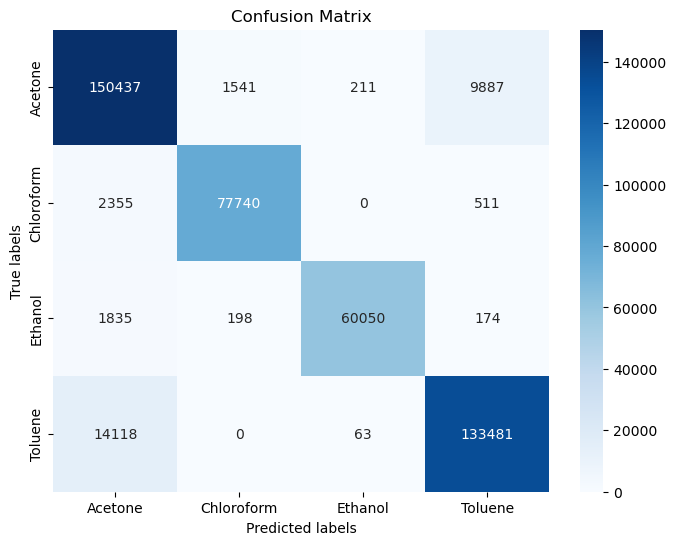
\includegraphics[width=0.8\linewidth]{Thesis Prashant//Images//Results/confusion_matrix_new_dataset.png}
    \caption{Confusion Matrix for trained neural networks on New Data set}
    \label{fig:enter-label}
\end{figure}
